% Chapter 1



\chapter{Literature Review} % Write in your own chapter title
\label{Chapter2}
\lhead{Chapter 2. \emph{Literature Review}} 
\section{Search strategy and selection criteria}
 This review aims to identify systems related to the automation of the nursing care workflow. Automation that has been adopted or can be adopted to assist nurses in routine tasks. Automation may be classical digitization methods or cutting-edge AI technology coupled with IoT to cover a plethora of tasks being performed by nurses.  
\subsection{Research Questions}
The review focuses on finding the market gap among top-notch systems and provides a way forward to improve and empower healthcare with technology. This review seeks to address the following research questions.
\begin{enumerate}
    \item What technologies and approaches have transformed nursing care workflow?
    \item What methods have been used for temporal action recognition?
\end{enumerate}
\subsection{Information sources}
To conduct a systematic literature review and draw a fair comparison between the existing cutting-edge Nursing Care Automation Systems, specific keywords must be used to search against databases. The databases used to search for relevant systems were Google Scholar, PubMed, IEEE Xplore, ScienceDirect, BMC Nursing, Springer Link, JAMIA, and Wiley Online Library. The databases were selected based on their content encompassing a vast majority of research literature closely related to technology and specifically to research in nursing. Searching different databases will ensure that no research work goes unnoticed and that the results are also accurate. Hence, we broaden our search while keeping it precise.
\subsection{Search strategy}
Before defining the keywords, a random search was conducted to identify systems for nursing care automation. To ensure that such articles were not missed, synonyms of keywords were used to search multiple databases. To finalize the keywords for searching nursing systems, a random search was conducted to specify the keywords that can be used to fetch articles discussing individual systems or review papers on single-task automation. This helps gather an initial search pool of keywords. Once again, using synonyms, the search field increased. Boolean AND and OR operators were used to form various combinations of keywords within categories. Wildcards and truncations were used with keywords. 

\subsection{Selection criteria}
Considering the wealth of research and experimentation spanning the past decade, evaluating the relevant systems in the last decade makes sense when comparing SOTA technologies being utilized in the nursing sector.
As the review is focused on systems that have been either adopted or are capable of being used in a clinical setting, the proposed and hypothesized systems have also been included. Systems that may automate a single nursing task have been included to develop a step-by-step flow of nursing system development.

\section{Related work}
The nursing care workflow as in figure \ref{nursing-time-distribution} consists of multiple activities. \cite{StudyForNurseTime} found that nurses spent approximately 37\% of their time on patient care and the remaining on medication, documentation, and communication. For nurses, documentation sources play a vital role in acquiring the necessary patient information. 
\begin{figure}[h]
\centering
\tikz{\pie[color = white]
    {37.6/Patient Care,
    35.4/Documentation,
    13.4/Care Coordination,
    9.3/Medication,
    5.3/Vital Signs Reading
    }
}%
 \caption{Fraction of Time Spent by a Nurse on Different Tasks of Nursing Care Workflow \cite{nursing-time}}
 \label{nursing-time-distribution}
\end{figure}
\cite{nursing-time} showed that nurses spend approximately 35\% of their time documenting. This shows that documentation is a major task for nurses, which if automated to some extent, may relieve some of the burden on nurses. Moreover, patient care consumes a major portion of the time spent by nurses with patients. Patient care involves assisting the patient and monitoring patient activity and vital signs. Figure \ref{fig:nursingacts} shows the nursing activities extracted from a study by \cite{nurse-activities}.
\begin{figure}
    \centering
    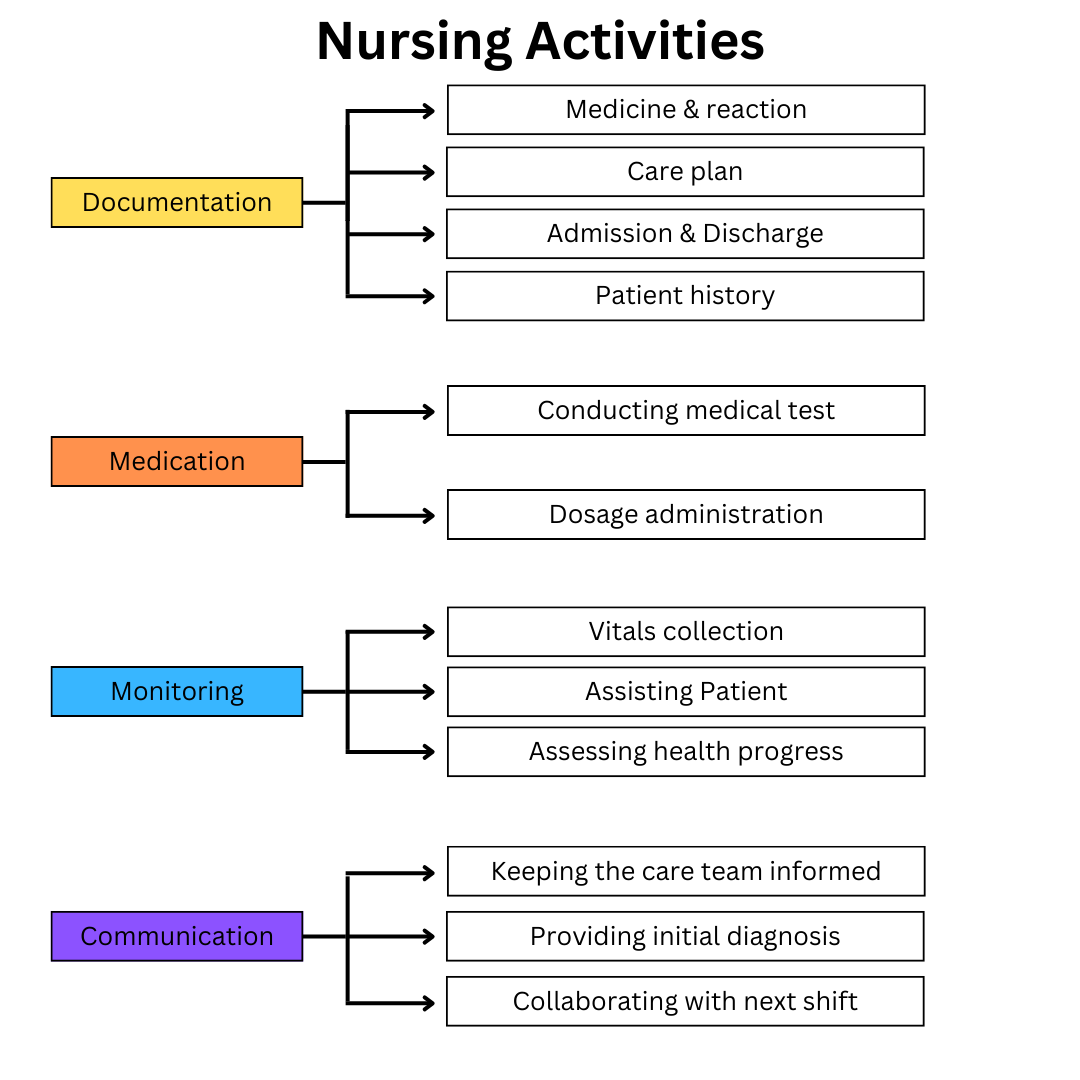
\includegraphics[width=1\linewidth]{images/Nursing Activities.png}
    \caption{Major Nursing Activities that may be Automated to an Extent}
    \label{fig:nursingacts}
\end{figure}
It shows how the nursing care workflow can be divided into 4 main categories. These are not the only activities as nurses are involved in logistics among other activities as well. The activities shown in the figure have been selected because they consume a major portion of a nurse's time.
\subsection{Digitization}
The first step towards any automation is converting the manual workflow and paperwork into digital format. Each step counts towards automation, setting up a path for future efforts to be streamlined. \cite{Study3} conducted an experimental study in 2003. They highlighted the limitations of traditional paper-based nursing records. They further emphasized the need for computerization of nursing records and proposed the use of a terminology-based ENR system. The study consisted of three phases: analysis of nursing notes, development of a terminology server and an ENR, and an evaluation of the system. Nursing notes were decomposed into phrases and cross-mapped with the International Classification for Nursing Practice (ICNP). The terminology server was developed to manage nursing concepts and phrases, whereas the user application system facilitated nursing note documentation. The system was evaluated in two Korean hospitals by 20 nurses documenting nursing notes for 57 patients.\\
Analysis of nursing notes revealed patterns reflecting the nursing care workflow, supporting the feasibility of structuring narrative nursing notes. A total of 14,727 phrases were used to document nursing notes. Among the 259 unique nursing concepts extracted, there were 237 unique phrases identified. The mean time required for documentation decreased significantly from 276s to 158s as users gained experience with the system. The results indicated that the ENR is indeed effective in a clinical setting. Nurses achieved a higher success rate and exhibited rapid adaptation over time. The findings underscore the potential of digital solutions like ENR systems to optimize nursing documentation, freeing up more time for direct patient care and improving patient outcomes. This study aligns closely with our research objectives of exploring automation technologies to enhance nursing care workflow and highlights the importance of digital transformation in healthcare.

% ---------------------------Usability Study-------------------------------------
In 2011 \cite{enr-usability} aimed to evaluate ENR systems and provide guidelines for further development of technologies in nursing. The study incorporated five key attributes specific to ENR systems for its usability evaluation: fluency of reporting practices, accuracy of documentation, adaptability, exploitation of documented information, and support for collaborative care.
The evaluation study was conducted in Finland in 2010, and involved four ENR systems used in various healthcare settings. Contextual interviews were conducted with 18 nurses from different organizations, focusing on documentation practices, practical exercises, and information exchange.
The study revealed that nurses preferred electronic documentation for its accessibility and potential for information reuse, but all evaluated systems exhibited usability problems. Documentation was time-consuming because of poor user interface design and complex interaction sequences. The systems did not align with the nurses' mental models, lacked support for structured templates and copy functionality, and required redundant data entry. Nurses reported difficulties in learning. Accessing and reading documented information was problematic, impacting collaborative care among healthcare professionals. 
The study emphasized the importance of aligning ENR systems with nursing practices and called for a conceptual redesign of these systems. These findings serve as a foundation for evaluating the current state of usability and informing future enhancements in ENR systems. This will become the foundation for the evaluation of our system.

% ---------------------------------Something--------------------------------------
\cite{emr-impact} investigated the impact of Electronic Medical Record (EMR) technology on nursing efficiency through a comprehensive literature review. Utilizing PubMed, Ovid, and general-purpose search engines, the researchers identified 23 relevant articles. By analyzing baseline measurements of nursing efficiency in using the Value Model Realization (VMR) Program, implemented by Texas Health Resources (THR), in hospitals before EMR conversion, the study provided valuable insights into the efficacy of EMR systems in optimizing nursing workflows. The study found that the nurses saved on average 73 minutes in normal wards and 50 minutes in ICUs during their 12-hour shift enabling them to support other initiatives. The study stressed the need for comprehensive understanding and coordination among disciplines for the efficient development of systems to support nursing. 

The studies show that an ENR is a practical solution for automation and it must be pursued but our approach incorporates a vision for activity recognition. To draw a fair comparison we must incorporate systems that automate nursing via sensors and vision. Activity recognition is a complex task. Several studies on major activity datasets for action recognition have been published. On the Kinetics-700 Dataset, a study \cite{InternVideo} achieved the highest accuracy of 84\%. They achieved 91.1\% top-1 accuracy on the kinetics-400 dataset and 77.2\% top-1 accuracy on the something-something v2 benchmark. \cite{ViT} integrated the vision transformer (ViT) and its variant UniformerV2, alongside additional local spatiotemporal modeling modules, to facilitate multi-level representation interaction. By taking advantage of both generative and discriminative self-supervised video learning they achieved 91.3\% accuracy on the kinetics-600 dataset whereas \cite{TubeViT-H} achieved the SOTA accuracy of 91.8\% on the same dataset. While conventional methods only initialize the linear classifier head for vision classification, \cite{ViT} leveraged the text encoder from pre-trained language models for visual recognition tasks. Replacing the classifier with knowledge from the pre-trained language model achieved SOTA. For ActivityNet, which is another popular human activity dataset, they achieved the highest accuracy of 96.9\%. This shows that there isn't a single approach to solving the problem of activity recognition and models have different accuracy when the dataset varies. All these approaches solve the problem of trimmed data. Trimmed data contains clips that are guaranteed to contain an activity within its short duration spanning a few seconds. The SOTA on untrimmed data for temporal activity recognition using the AR@50 metric is 64.28\% on the Thumos14 dataset. The activity in our use case needs to be detected, localized, and recognized for patients in hospital wards therefore an AR@5 metric is a more cohesive choice. With such a metric the accuracy of the existing models drops significantly to a staggeringly low 33\%. Several studies have attempted to recognize activities of daily living.
\subsection{Sensor-based patient monitoring}
\cite{robot-impact} explored the utilization of robots and automated devices in nursing care. The focus was on their impact on nurses' work efficiency and patient outcomes. Most of the 25 studies reviewed were conducted in hospital settings, with some in elderly care centers or nursing homes. The technologies used were categorized into algorithm-based methods, sensor technology, and automatic robotic devices. The most extensive application was in medication care, where robots were employed for automated dispensing systems and bar code-assisted medication administration. These interventions significantly reduced medication errors, improved nurses' working time, and enhanced overall satisfaction. Additionally, robots were utilized for patient monitoring and nursing treatments, showing promising results in reducing nurses' workload and improving patient safety. Use of robots and IoT medical devices can become an extension of our work to better optimize nursing care workflow.

%------------------------SVDD Implementation------------------------
\cite{Study7} proposed a situation-aware abnormality detection system based on Support Vector Data Description (SVDD) for elderly people. The authors emphasized the significance of abnormal activity detection in elderly care as it can help predict diseases and provide timely support. This study aimed to detect abnormal activities in specific situations by analyzing features and designing a zone-based situation detection system. SVDD is employed to detect abnormal activity based on the designed features. The feasibility and accuracy of the proposed method are experimentally evaluated.
The hardware used in the system includes a U-tile sensor network for precise location tracking and a smart plug to monitor home appliance status. The U-tile sensor network utilizes pressure sensors and RFID antennas embedded under the floor to track the position of elderly individuals. The home setup is divided into various zones. The situation is determined based on the zone, status of related devices, actions of the elderly personnel, and environmental factors. The results of the experiments indicate that the system achieves a high accuracy in detecting situations and abnormal activities, with only a few errors detected. The system successfully detected all abnormal activities and provided warning services to remote family members. Future plan is to implement the system in a hospital ward and evaluate its performance in detecting other situations and abnormal activities.

\cite{DDPM} proposed a system to monitor a patient’s condition by monitoring the body temperature and pulse rate. It consists of pulse rate monitoring software and a wearable device that can measure a subject’s temperature and pulse rate using a fingertip only. The wearable device can record the measurement data and interface to a desktop via an Arduino microcontroller. It provides a cost-effective solution due to limited hardware requirements for patient vitals monitoring but is limited to temperature and pulse rate only. In another experimental study, \cite{necklace-sensor} proposed a sensor-based wearable device that allows continuous patient monitoring, specifically in a nursing home setting. The device automatically provides alarms to caregivers based on biosignals measured by sensors integrated into a necklace worn by each patient. The device detects the heart rate, involuntary falls, and the location of the patient within a building. It also has a manual call button. \cite{arduino-remote-monitoring} proposed a framework that integrates web services with multiple sensors controlled by Arduino Uno. Four types of sensors were used to monitor the patient's vital signs such as electrocardiogram (ECG), body temperature, pulse rate, and oxygen in blood (SPO2). The system improves real-time data collection, eliminates manual data gathering, and enables the monitoring of a large number of patients at the cost of integrating sensors with a singular interface chip called an eHealth shield, which then connects with Arduino Uno to send the data to a web service. \cite{jamjoum} proposed a portable patient monitoring system. Blood oxygen saturation levels, electrocardiogram, heart rate, and body temperature were the main vital signs measured. Each vital sign was captured using a sensor connected to a microcontroller with a built-in wireless communication module. The micro-controller processes the vital signs' data and uploads it to the cloud. The user interface was built on three platforms: an Android application, a website, and a hand-held module based on Raspberry Pi. The system captures vital signs and uploads the readings in real-time, enabling medics to monitor and assess a patient's medical condition remotely. Real measurements were taken using the system and compared to readings obtained using appropriate devices in a medical clinic. The results showed that the system could capture the vital signs with a deviation of less than 10\% from the referenced readings. This architecture makes it very suitable for long-distance online patient monitoring. This approach removed the need for an eHealth shield interface that was used in the previous study by Theses studies provide an important insight into how our prototype can be extended to incorporate sensors measuring vital signs.

\cite{smartphone} presented a self-learning scheme for smartphone-based activity recognition aimed at enhancing medical monitoring for patients, particularly postoperative individuals, using data collected from common motion sensors in smartphones. The purpose of the study is to develop an adaptive system capable of recognizing both known and unknown activities without prior knowledge of the latter. The methodology involves preprocessing sensor data to eliminate orientation influence, extracting robust features, and employing a self-learning framework for activity recognition. The self-learning scheme dynamically clusters unknown activity data and assigns new category labels, which are then merged into the training dataset to improve recognition accuracy. Experimental results, conducted with data from postoperative patients performing six labeled daily activities, demonstrate that the proposed scheme achieves high accuracy, surpassing 80\% even when faced with multiple types of unseen activities. The study contributes to the field by introducing a comprehensive self-learning framework for activity recognition using smartphone sensors, aligning with the broader goal of advancing mobile health applications for patient monitoring.

\subsection{Vision-based automation patient monitoring}
A range of studies have explored real-time patient activity recognition using cameras. \cite{Study6} proposed a context-aware human activity recognition (HAR) system using a depth camera to improve the privacy and security of patients. With the use of depth cameras, the image becomes noisy; thus the authors introduce a novel feature selection technique to extract and select the most relevant features for activity recognition. The proposed system is evaluated using hidden Markov models (HMM) and compared to existing works that use depth cameras.\\
The proposed approach starts with an empty model, adding and removing variables based on important tests such as the partial F-test. The alpha-to-enter and alpha-to-eliminate values control the inclusion and exclusion of variables. The step-wise regression built a model that initially includes all independent variables and then eliminates those that are not statistically significant. The proposed approach for feature extraction and selection aims to reduce the feature space to a constrained number of features. It uses FLD and forward-backward regression algorithms.
The authors train and test the proposed approach offline. Future research should implement the proposed approach in an actual clinical setting. The accuracy achieved was not near SOTA techniques that do not cater to privacy. Nevertheless, it has set a benchmark for privacy in activity recognition. This study has shown an important aspect of security and privacy that needs to be considered while monitoring patients. This introduces another challenge for future work, considering that feature extraction through visual input can be cumbersome and significantly reduce accuracy.

\cite{UET-Study} discussed the problem of recognizing abnormal human activities in videos of patients. The authors proposed a multi-class abnormal action detection system that utilizes the You Only Look Once (YOLO) network as a backbone convolutional neural network (CNN) model. The CNN model was trained using a large dataset of patient videos constructed by them. Each frame was labeled. There were 23,040 labeled images of patients’ actions for 32 epochs.
The proposed approach involves dividing the videos into segments and then applying the trained CNN model for classification prediction on each segment. The confidence and prediction scores are calculated based on Intersection over Union (IOU) for all classes. Evaluation metrics, such as accuracy, precision, recall, and F1-score, are then computed into a confusion matrix to assess the performance of the system. The proposed approach achieves a high accuracy of 96.8\% for abnormal action recognition, with an improved F1-score of 89.2\% compared with SOTA techniques. The authors also highlight the limitations of the YOLO model, particularly its inability to predict the number of objects and handle small objects. The paper suggests future work to extend the system's capabilities for handling multiple objects and individuals in real-world scenarios. 
\cite{fuzzy} proposed a fuzzy logic classifier for elderly patient fall detection. The proposed approach involves creating a home surveillance system using ordinary webcams. These webcams track subject movement, and the video stream is processed in MATLAB. After background subtraction and cleaning, relevant parameters (such as center of mass, aspect ratio, body speed, and face speed) are extracted from the image sequences. The system includes feature extraction and classification of events. The authors use a fuzzy logic classifier to tabulate these events according to two decisions: FALL or NON-FALL. The experimental results proved that they could discriminate a falling event from a non-fall situation by combining the different parameters. The authors achieved results with a sensitivity of 92.7\% and a specificity of 99.1\% for fall detection. This helps us extend our future plans to abnormal activity detection using their specific fuzzy logic classifier. 

\cite{neural-network} developed a video-based framework for real-time activity recognition. Simple motion features are modeled over time and classified into different activity levels using a neural network. For the experiments, the Sheffield Activities of Daily Living dataset is used where each activity is simulated within a simulated assisted living environment under two different illumination conditions. Their experiments show that the detection rate for each of the activity levels is well above 80\% and the detection time is approximately 30 seconds. The fact that the dataset contains simulated activities, may not work so well in a real clinical setting and so there is a need to test this approach in a real-world scenario.

\cite{wearable-cams1} presented a novel approach for activity recognition using video data captured by a wearable camera, to assist individuals living with disabilities or the elderly in their daily activities. The purpose of the study is to develop a system capable of remotely identifying specific activities such as drinking, walking, going upstairs, and going downstairs. The methodology involves extracting features using optical flow and applying classifiers such as k-Nearest Neighbors (k-NN), LogitBoost, and Support Vector Machine (SVM), followed by smoothing using the Hidden Markov Model (HMM). Results indicate that average pooling significantly enhances performance, with SVM (RBF kernel) achieving the highest accuracy of 76.7\%. Furthermore, incorporating multi-activity videos into the training dataset improves classification accuracy by an average of 6.2\%. Figures and values provided in the paper illustrate the performance of different classifiers and the impact of feature extraction methods and training data on accuracy. This research provides insights into the development of a wearable camera-based system for activity recognition, which aligns with the broader goal of leveraging technology to assist individuals with disabilities or cognitive impairments in their daily lives.

\cite{wearable-cams2} proposed a novel method for activity recognition in Ambient Assisted Living applications, focusing on analyzing recordings of daily living captured by wearable cameras. The approach involves constructing discriminant object-centric motion descriptors to represent micro-actions within the viewpoint of the action maker, aiding in defining the performed activity. The study utilizes deep learning techniques for object detection and motion analysis, incorporating both Histograms of Optical Flow (HOF) and Motion Boundary Histogram (MBH) descriptors. The results on the ADL dataset show that the proposed method with the MBH descriptor outperforms state-of-the-art approaches in activity recognition.. The paper contributes to the field of activity recognition from egocentric videos, offering insights into behavior monitoring and health applications, which aligns with our future focus on leveraging wearable technology for assisted living environments. 

\section{Current State-of-the-Art}
Aside from systems being researched, some software solutions are being used in the healthcare industry. Some of the popular solutions are listed below.
\subsection{MyChart by Epic}
MyChart lets you see your medications, test results, upcoming appointments, medical bills, and price estimates. It can be integrated with other EHRs such as Cerner Aware to transfer data. It is more patient-oriented and focuses on providing reminders and medication to the patient while providing analytics of medical history only instead of real-time vitals.
\subsection{Cerner}
Cerner Melior is a comprehensive medical record system developed in collaboration with Swedish healthcare. The system provides support for patient care and is used in 32 hospitals across Sweden. It provides real-time vital monitoring by integrating medical devices with a comprehensive dashboard.
Cerner Millennium is aimed at helping in documentation and assessing critical patient data, streamlining workflows, and helping to improve both patient safety and the overall patient experience. It is a little more advanced than its Melior counterpart as it provides an additional feature of patient vitals analytics.
At the heart of Cerner, the Cerner Aware is the main product with the most features that Cerner offers. An environment for multiple EHR integrations. It uses medical Device integration to capture real-time vitals and provide data analytics.
\subsection{MEDITECH Expanse}
MEDITECH Expanse is a web-based EHR. Expanse goes beyond basic record-keeping by offering features that improve clinical workflows and patient care.  Clinicians can leverage mobile capabilities to access patient charts and documentation at the bedside, while features like decision support tools and integrated genomics can aid in informed treatment decisions.  Expanse focuses on patient engagement with patient portal access and aims to reduce the administrative burden for healthcare staff through its user-friendly interface.
\subsection{AthenaOne}
AthenaHealth offers a cloud-based solution AthenaOne, designed to improve efficiency and patient care.  Nurses benefit from features like customizable templates and macros to reduce documentation time, athenaCommunicator for secure patient engagement, and real-time access to patient data through its' app.  AthenaHealth focuses on user experience with features like intuitive workflows and easy navigation, aiming to minimize time spent on administrative tasks and maximize time spent with patients.
\subsection{eClinical Works}
eClinicalWorks is a cloud-based EHR designed to streamline workflows for healthcare providers. This translates to features such as AI-powered documentation tools that simplify note-taking, improved access to patient data anywhere and anytime, and communication functions to collaborate with doctors and patients. eClinicalWorks goes beyond basic EHR by incorporating advanced AI features like "Sunoh" which converts conversations to documentation and an "AI Assistant" for streamlining tasks.
\subsection{PointClickCare}
PointClickCare serves as a comprehensive EHR solution, granting healthcare providers easy access to residents' and patients' medical records, facilitating streamlined medication management, personalized care plans, and efficient billing and financial management. The system also aids in staff scheduling and training, offers health analytics insights, and fosters seamless communication among care teams. With its user-friendly interface and integration capabilities, PointClickCare ensures regulatory compliance, supports remote access, and can be tailored to different healthcare settings, ultimately enhancing the overall quality of care provided.

\subsection{Vocera}
Vocera's solutions for smart nursing involve the use of wearable devices and mobile apps. It allows nurses to communicate with each other and with patients in a voice-activated manner. The Collaboration Suite delivers real-time situational awareness. Vocera Edge is a cloud-based communication solution for smartphones that allows nurses to quickly recognize and respond to changes in a patient's status. It enables them to document EHR, receive filtered alarm notifications, view vital signs, and send secure messages tagged with patient data and care team information.
\subsection{Closer - Elderly Smart Home}
A smart home nursing solution that uses depth sensors to detect abnormal activity. It informs the caretakers and remotely located nurses. Comes embedded with an EHR system that provides real-time health conditions to caretakers. It doesn't use any RGB cameras and is integrated with medical devices to extract vitals. 
\subsection{Smart Peep}
It utilizes computer vision to detect abnormal behavior in real-time such as falls, motionless anomalies, and unusual absences. It then alerts the caretakers to take action. It is more home-oriented and does not involve any vitals monitoring. 
\section{Comparison}
Table \ref{tab: comparison} presents a comparison of the relevant products in the market. Each system is either an EHR, a Medicine Management System, or a Telehealth system. They either utilize their own custom-made hardware vital collection devices or integrate them with existing medical devices. 
The top 3 have been selected specifically which take up roughly 70\% of the market. Studies have shown that nurses tend to prefer paper-based documentation over electronic systems simply because they fail to provide the best and easiest user interface and experience. Some of the following products provide a cluttered but comprehensive dashboard with low personalization.  The products also fail to provide nurses with task organization and prioritization. They also integrate medical devices which is an accurate form of data collection but is costly.

\begin{table}[h]
\centering
\caption{Comparison of Features Offered by Popular Healthcare Solutions}
 \resizebox{\columnwidth}{!}{%
 \renewcommand{\arraystretch}{1.5} 
            \begin{tabular}{|m{3cm}|>{\centering\arraybackslash} m{2.5cm}|>{\centering\arraybackslash} m{2.5cm}|>{\centering\arraybackslash} m{2cm}|>{\centering\arraybackslash} m{2cm}|>{\centering\arraybackslash} m{2cm}|>{\centering\arraybackslash} m{2.5cm}|}
            \hline
            \textbf{\large Products} & \textbf{Activity recognition} & \textbf{Realtime monitoring} & \textbf{Task alerts} & \textbf{Detailed dashboard} & \textbf{Patient Analytics}& \textbf{Forecasting} \\
\hline
 \large Epic  & x & \checkmark & \checkmark & \checkmark & \checkmark & x \\
\hline
\large Cerner  & x & \checkmark & \checkmark & \checkmark & \checkmark & x \\
\hline
\large Meditech  & x & \checkmark & x & \checkmark & \checkmark & x \\
\hline
\large Athena health  & x & \checkmark & x & \checkmark & x &x\\
\hline
\large eClinical works & x & \checkmark & x & \checkmark & x & x\\
\hline
\large Point click care  & x & \checkmark & \checkmark & \checkmark & x & x\\
\hline
\large Vocera  & x & \checkmark & \checkmark & x  &  \checkmark & x\\
\hline
\large Closer  & \checkmark & \checkmark & x & x & \checkmark & x \\
\hline
\large Smart Peep  & \checkmark & \checkmark & x & \checkmark & \checkmark & x \\
\hline
\large Nursing portal & \checkmark & \checkmark & \checkmark & \checkmark & \checkmark & \checkmark \\
\hline
\end{tabular}
}
\label{tab: comparison}
\end{table}
\section{Discussion}
In examining the literature about the transformation of nursing care workflow, several key technological advancements emerge. Digitization, exemplified by studies such as Cho et al. (2003) and Viitanen et al. (2011), showcases the shift from manual paper-based records to electronic nursing records (ENR) systems. These systems not only optimize nursing documentation but also significantly reduce documentation time, as evidenced by Cho et al.'s findings. However, challenges in usability and alignment with nursing practices, highlighted by Viitanen et al., underscore the need for user-centered design in ENR implementation. Additionally, the integration of electronic medical record (EMR) systems, as explored by Thompson et al., demonstrates substantial time savings for nurses and emphasizes the importance of interdisciplinary coordination in technology adoption. Concurrently, sensor-based patient monitoring technologies, as investigated by Kangasniemi et al. and others, offer promising avenues for improving medication administration, patient monitoring, and fall detection, thus reducing nurses' workload and enhancing patient safety. Regarding temporal action recognition methods, studies by Siddiqi et al., Gul et al., and Zhan et al. reveal innovative approaches using depth cameras and wearable cameras for real-time patient activity recognition, addressing privacy concerns and improving monitoring accuracy. Looking forward, integrating these technologies into nursing workflows holds significant potential for optimizing patient care and informing future research endeavors in healthcare innovation.

Studies show conflicting results at times when ENRs are used. It cannot be conclusively said that the results from the study conducted by \cite{Study3} will be sustainable on a larger scale. The scope of the study was limited to two Korean hospitals and 20 nurses. They may have a higher success rate and improved patient outcomes, but the results can be detrimental if the software is not designed keeping the nurses' mental model in mind. Usability has been a major concern of the nurses so any future system that is developed should be strictly cohesive with the nursing care workflow while allowing for personalization of its interface as well. The application should be easy to navigate. 

Although a novel approach, there were issues with the proposed methodology of \cite{Study7}. While SVDD is a powerful tool for anomaly detection, its performance could be influenced by the choice of features and the quality of the dataset used for training. Without a thorough discussion of feature selection and dataset characteristics, the robustness and generalizability of the proposed method remain unclear. Additionally, the study relies on hardware components such as U-tile sensor networks and smart plugs for data collection, which may introduce practical challenges related to installation, maintenance, and scalability, particularly when deploying the system in real-world healthcare environments. 

While Azizulkarim et al's system offers simplicity and affordability, it is limited to monitoring only two vital signs. Hameed et al's proposed integration with a singular interface chip may pose scalability challenges. In contrast, Jamjoum et al. presented a portable patient monitoring system capturing vital signs like blood oxygen saturation levels, ECG, heart rate, and body temperature, with data uploaded in real-time to facilitate remote monitoring by healthcare providers. This system, leveraging wireless communication and cloud-based storage, offers a scalable solution suitable for long-distance patient monitoring.
The monitoring and logging of a patient's activity and vital signs is the second most important task. It was noted that using depth sensors instead of cameras for activity recognition may result in lower accuracy of temporal activity recognition, particularly when considering privacy concerns. Systems that have higher accuracy use a multitude of sensors such as floor pressure tiles and IoT home appliances to gather as much information about the patient and location to access the patient status. This leads to an expensive solution and requires specialized hardware which may not be as readily available as cameras are. Some systems that utilize only cameras and achieve high accuracy are slow in their response failing to achieve true real-time monitoring. 

In a clinical setting, a system with minimal lag must be put in place that leverages the existing and prevalent infrastructure to provide a cost-effective and feasible solution that provides patient activity recognition, forecasting, assistance with nursing care workflow, and a comprehensive patient analytical dashboard similar to that found in EHR solutions today. A major amount of research needs to be conducted in temporal activity recognition and forecasting patient activities. 


% Write in your chapter title to set the page header